% Options for packages loaded elsewhere
\PassOptionsToPackage{unicode}{hyperref}
\PassOptionsToPackage{hyphens}{url}
%
\documentclass[
]{article}
\usepackage{lmodern}
\usepackage{amsmath}
\usepackage{ifxetex,ifluatex}
\ifnum 0\ifxetex 1\fi\ifluatex 1\fi=0 % if pdftex
  \usepackage[T1]{fontenc}
  \usepackage[utf8]{inputenc}
  \usepackage{textcomp} % provide euro and other symbols
  \usepackage{amssymb}
\else % if luatex or xetex
  \usepackage{unicode-math}
  \defaultfontfeatures{Scale=MatchLowercase}
  \defaultfontfeatures[\rmfamily]{Ligatures=TeX,Scale=1}
\fi
% Use upquote if available, for straight quotes in verbatim environments
\IfFileExists{upquote.sty}{\usepackage{upquote}}{}
\IfFileExists{microtype.sty}{% use microtype if available
  \usepackage[]{microtype}
  \UseMicrotypeSet[protrusion]{basicmath} % disable protrusion for tt fonts
}{}
\makeatletter
\@ifundefined{KOMAClassName}{% if non-KOMA class
  \IfFileExists{parskip.sty}{%
    \usepackage{parskip}
  }{% else
    \setlength{\parindent}{0pt}
    \setlength{\parskip}{6pt plus 2pt minus 1pt}}
}{% if KOMA class
  \KOMAoptions{parskip=half}}
\makeatother
\usepackage{xcolor}
\IfFileExists{xurl.sty}{\usepackage{xurl}}{} % add URL line breaks if available
\IfFileExists{bookmark.sty}{\usepackage{bookmark}}{\usepackage{hyperref}}
\hypersetup{
  hidelinks,
  pdfcreator={LaTeX via pandoc}}
\urlstyle{same} % disable monospaced font for URLs
\usepackage[left = 20mm, right = 20mm, top = 10mm, bottom =
45mm]{geometry}
\usepackage{longtable,booktabs}
\usepackage{calc} % for calculating minipage widths
% Correct order of tables after \paragraph or \subparagraph
\usepackage{etoolbox}
\makeatletter
\patchcmd\longtable{\par}{\if@noskipsec\mbox{}\fi\par}{}{}
\makeatother
% Allow footnotes in longtable head/foot
\IfFileExists{footnotehyper.sty}{\usepackage{footnotehyper}}{\usepackage{footnote}}
\makesavenoteenv{longtable}
\usepackage{graphicx}
\makeatletter
\def\maxwidth{\ifdim\Gin@nat@width>\linewidth\linewidth\else\Gin@nat@width\fi}
\def\maxheight{\ifdim\Gin@nat@height>\textheight\textheight\else\Gin@nat@height\fi}
\makeatother
% Scale images if necessary, so that they will not overflow the page
% margins by default, and it is still possible to overwrite the defaults
% using explicit options in \includegraphics[width, height, ...]{}
\setkeys{Gin}{width=\maxwidth,height=\maxheight,keepaspectratio}
% Set default figure placement to htbp
\makeatletter
\def\fps@figure{htbp}
\makeatother
\setlength{\emergencystretch}{3em} % prevent overfull lines
\providecommand{\tightlist}{%
  \setlength{\itemsep}{0pt}\setlength{\parskip}{0pt}}
\setcounter{secnumdepth}{-\maxdimen} % remove section numbering
\usepackage{fancyhdr, graphicx, eurosym, booktabs, xcolor, lastpage} \pagestyle{fancy} \fancyhf{} \addtolength{\headheight}{2.5cm} \fancyheadoffset{10mm} \lhead{\IfFileExists{logo.png}{\includegraphics[height = 2cm]{logo.png}}} \lfoot{Page \thepage~of~\pageref{LastPage}} \fancypagestyle{plain}{\pagestyle{fancy}} \renewcommand{\headrulewidth}{0pt} \setlength{\headsep}{12mm} \usepackage{titling} \usepackage{booktabs} \usepackage{multicol} \usepackage{caption} \setlength{\belowcaptionskip}{0pt plus 1pt minus 1pt} \usepackage{hyperref} \hypersetup{urlcolor = cyan}
\ifluatex
  \usepackage{selnolig}  % disable illegal ligatures
\fi

\author{}
\date{\vspace{-2.5em}}

\begin{document}

\(~\)

\vspace{5ex}
\begin{center}\textsc{\huge Calibration Certificate Information}\end{center}
\vspace{8ex}

\textbf{\Large Calibrating Laboratory}\newline \textbf{Adress}
\vspace{4ex}

\hypertarget{certificate-number-4637}{%
\subsection{\texorpdfstring{Certificate number:
\textbf{4637}}{Certificate number: 4637}}\label{certificate-number-4637}}

\(\hrulefill\)

\(~\)

\begin{tabular}{@{$\qquad\qquad$}rp{0.7\linewidth}}
 \textbf{\large Object to calibrate:}&\textbf{\large Non Automatic Weighing Instrument (NAWI)}\\[3ex]
 \textbf{Identification:}&Balanza Mettler Toledo XPE 205\\
 \textbf{Serial:}&B743848411 / AF-07090\\
 \textbf{Calibration date:}&2020-07-16\\
 \textbf{Calibration place:}&Bogotá - Colombia.  Avenida Carrera 50 No. 26 - 55 Interior 2\\[2ex]
 \textbf{Responsible person:}&Ingeniero Jhon Alexander Barreto Gutiérrez\\
                     & Físico Jorge Daniel Garcia Benavides\\
                     &\\[2ex]
\multicolumn{2}{@{}l}{\textit{Environmental conditions during calibration}}\\
\textbf{Ambient temperature:} & 19.85 $^oC$\\
\textbf{Barometric pressure:} & 751.75 hPa\\
\textbf{Relative humidity:}   & 46.05 \%\\
\end{tabular}

\(~\)

\(\hrulefill\)

\vspace{1ex}

\hypertarget{nawi-description}{%
\subsection{NAWI description}\label{nawi-description}}

\begin{tabular}{@{$\qquad\qquad\qquad$}rrl}
 \textbf{ Maximum load:}&\textbf{220} & mg\\
 \textbf{ Minimum load:}&\textbf{0.01} & mg\\
 \textbf{ Readability:} &\textbf{0.01} & mg\\
\end{tabular}

\(~\)

\(\hrulefill\)

\begin{flushright}
  \texttt{masscor App Version: 0.1.12}
  
  \texttt{\url{http://186.155.29.169:3838/masscor/}}
\end{flushright}

\clearpage

\hypertarget{repeatability-test-results}{%
\subsection{Repeatability test
results}\label{repeatability-test-results}}

\begin{longtable}[]{@{}lrrr@{}}
\caption{Repeatability test data. Units: {[}g{]}}\tabularnewline
\toprule
& Load No.~1 / g & Load No.~2 / g & Load No.~3 / g\tabularnewline
\midrule
\endfirsthead
\toprule
& Load No.~1 / g & Load No.~2 / g & Load No.~3 / g\tabularnewline
\midrule
\endhead
Ind.1 & 0.00999 & 99.99997 & 199.99995\tabularnewline
Ind.2 & 0.00999 & 100.00001 & 200.00000\tabularnewline
Ind.3 & 0.00999 & 99.99998 & 199.99998\tabularnewline
Ind.4 & 0.01000 & 99.99998 & 199.99999\tabularnewline
Ind.5 & 0.01001 & 99.99997 & 199.99996\tabularnewline
Ind.6 & 0.01000 & 99.99998 & 199.99996\tabularnewline
Ind.7 & 0.01001 & 99.99997 & 199.99996\tabularnewline
Ind.8 & 0.01001 & 99.99996 & 199.99997\tabularnewline
Ind.9 & 0.01000 & 99.99999 & 199.99995\tabularnewline
Ind.10 & 0.01001 & 99.99996 & 199.99996\tabularnewline
. & & &\tabularnewline
Load & 0.01 & 100.00 & 200.00\tabularnewline
Standard.deviation & 8.8e-06 & 1.5e-05 & 1.7e-05\tabularnewline
\bottomrule
\end{longtable}

\(\hrulefill\)

\hypertarget{excentricity-test-results}{%
\subsection{Excentricity test results}\label{excentricity-test-results}}

\begin{minipage}{.3\textwidth}
  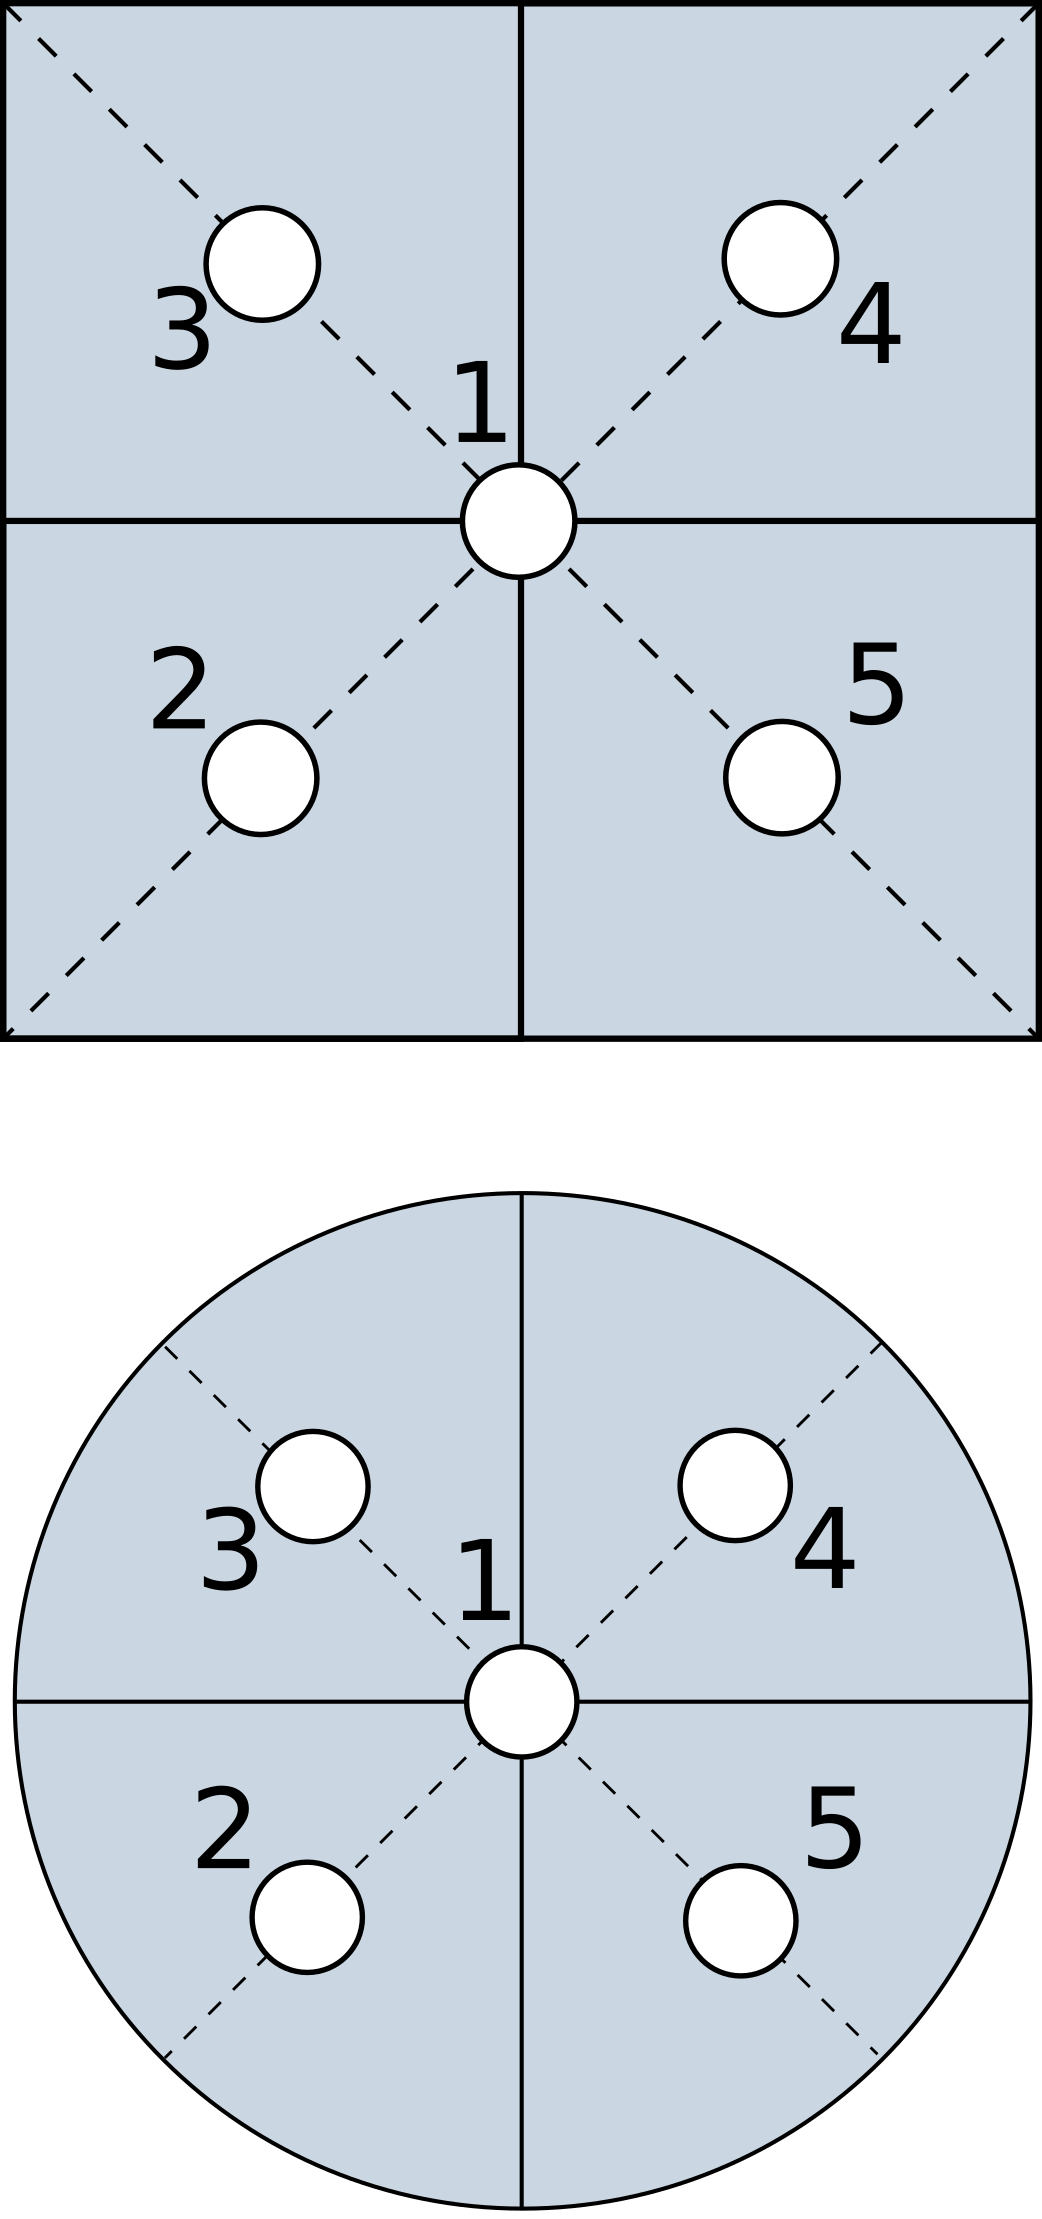
\includegraphics[width = 3cm]{eccen.png}
\end{minipage}
\begin{minipage}{.5\textwidth} 
    \captionof{table}{Eccentricity test results}
    \begin{tabular}{c r r}\toprule
    \textbf{Position} & \textbf{Indication / g} & \textbf{Difference / g}\\\midrule
    1 (Central position) & 99.99997 & -\\
    2 & 99.99996 & -0.00001\\
    3 & 100.00003 & 0.00006\\
    4 & 99.99998 & 0.00001\\
    5 & 99.99994 & -0.00003\\\midrule
    \multicolumn{2}{c}{\textbf{Maximum difference}}&0.00006\\\bottomrule
    \end{tabular}
\end{minipage}

\(~\)

\(\hrulefill\)

\clearpage

\hypertarget{indication-error-test}{%
\subsection{Indication error test}\label{indication-error-test}}

\begin{figure}
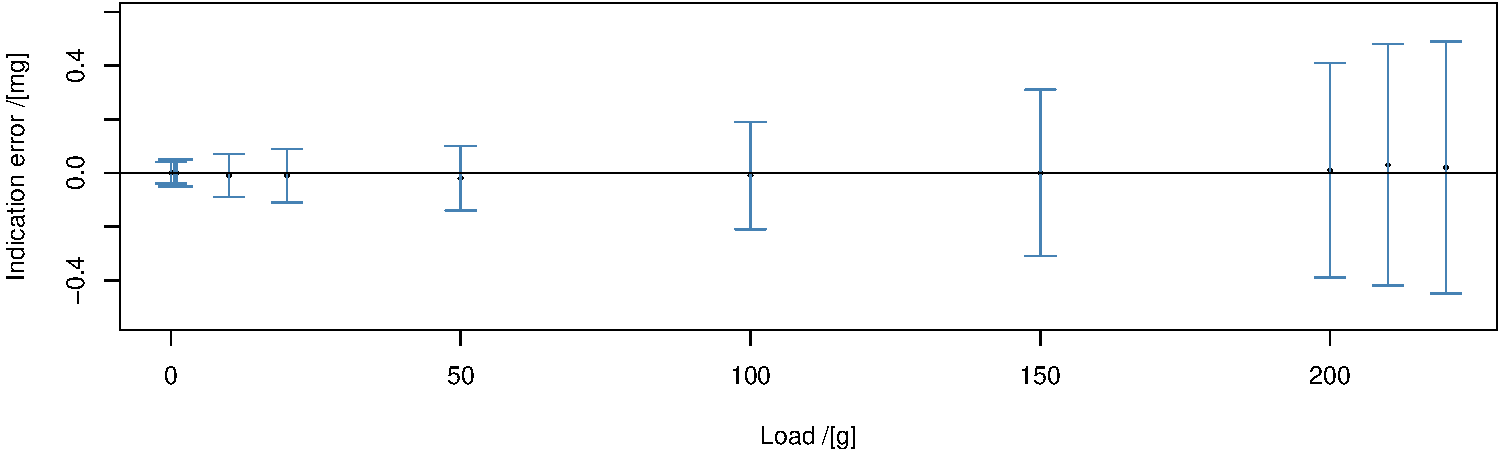
\includegraphics[width=1\linewidth]{Human_Readable_CC_files/figure-latex/unnamed-chunk-2-1} \caption{Indication error plot for the NAWI.}\label{fig:unnamed-chunk-2}
\end{figure}

\begin{longtable}[]{@{}rrr@{}}
\caption{Indication error test results}\tabularnewline
\toprule
Load / g & Error / mg & Uncertainty / mg\tabularnewline
\midrule
\endfirsthead
\toprule
Load / g & Error / mg & Uncertainty / mg\tabularnewline
\midrule
\endhead
0.01 & 0.00 & 0.020\tabularnewline
0.5 & 0.00 & 0.025\tabularnewline
1 & 0.00 & 0.025\tabularnewline
10 & -0.01 & 0.040\tabularnewline
20 & -0.01 & 0.050\tabularnewline
50 & -0.02 & 0.060\tabularnewline
100 & -0.01 & 0.100\tabularnewline
150 & 0.00 & 0.155\tabularnewline
200 & 0.01 & 0.200\tabularnewline
210 & 0.03 & 0.225\tabularnewline
220 & 0.02 & 0.235\tabularnewline
Uncertainti & es correspond & to expanded\tabularnewline
\bottomrule
\end{longtable}

\(\hrulefill\)

\clearpage

\hypertarget{comments-section}{%
\subsection{Comments section}\label{comments-section}}

This calibration certificate documents the traceability to national
standards, which realize the units of measurement according to the
International System of Units (SI). The results of this certificate are
related to the calibrated object. \vspace{2ex}

For the calibration is used the method of direct comparison with
standard weights, in accordance with the document ``Guidelines on the
Calibration of Non-Automatic Weighing Instruments'' EURAMET Calibration
Guide No 18 version 4.0 (11/2015). The following tests applies:
eccentricity, it determines the difference of indication of the
instrument with load in peripheral positions, as opposed to the position
in center of the load receptor. Repeatability, to quantify the
difference between the results of several weighing ones of the same load
when it is deposited several times and of practically identical form on
the load receptor and error of indication, considers the performance of
the instrument in the total range of measurement \vspace{3ex}

Review in a periodic way the behavior of the balance by means of control
with calibrated weights. If the balance is moved to another location
after the calibration are likely to alter performance of the balance and
may invalidate the calibration. The conformity of the equipment is
responsibility of the user according to the use and tolerances
established in the processes. Internal adjustment was made to the
balance.

\end{document}
